\chapter{Conclusion} \label{ch:discussion}

The work documented in this report was performed for two reasons. One was to
investigate \ac{BBCEAS} as an experimental technique, and to explore possible
modifications that would increase the sensitivity and repeatability of spectra
measured from a \ac{BBCEAS} setup. This technique was then used for the second
piece of work investigating the electronic transitions of aqueous europium and
what kind of ways \ac{BBCEAS} and europium could be combined.

The results obtained from investigating \ac{BBCEAS} are promising.
A reliable way of calculating and visualising error was crafted in
section~\ref{subsec:ceas_error}, and from creating the layout in
section~\ref{sec:optical_layout}, potential improvements were identified. In
addition, the effects of several sources of error were investigated in chapter
~\ref{ch:cal}. Through this investigation, a new file format named
\emph{CamTIFF} and a spectroscopic software suite called \emph{Apollo} were
created to simplify experimental design and work.

Building on this \ac{BBCEAS} framework, absorption spectra of europium
ions were detected to validate previous results in the literature,
as well as to investigate the potential uses of aqueous europium. A
theoretical understanding of europium's electronic configuration and the
implications of this to the observed absorption spectra were investigated in
chapter~\ref{ch:eu_theory}, and preliminary absorption spectra were obtained
in chapter~\ref{ch:eu_exp}.



\section*{Future Work}

\acl{BBCEAS} is a simple spectroscopic technique that in most cases is
used as a way to measure the concentration of an analyte in a solution.
This description tends to minimise a technique that can offer a greater
understanding of difficult theoretical and experimental questions. \ac{BBCEAS}
can probe electronic transitions that are otherwise impossible to detect with
other absorption techniques, and its spectrally wide results can be used to
understand the longevity of an excited state. This information can be used to
create efficient assays that provide solution specific spectroscopic values
that can be used not only to determine the concentration of an analyte but
to identify molecules in a solution that would otherwise be difficult or
impossible with other spectroscopic methods. In addition, the simplicity of
\ac{BBCEAS} allows it to be easily commercialised into a small, cheap and yet
potent form factor.

%\begin{wrapfigure}{o}{\marginspace}
%\begin{center}
%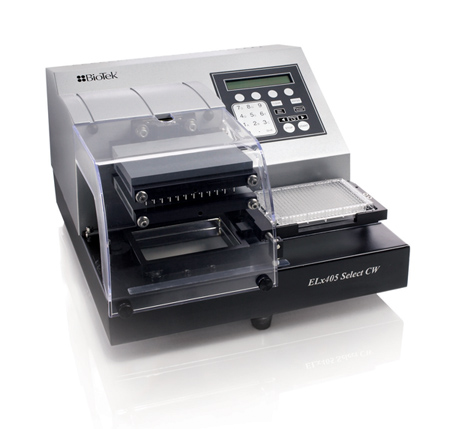
\includegraphics[width=\marginspace]{figures/microtiter_machine.jpeg}
%\end{center}
%\emph{\footnotesize{ A potential automatic protein assay machine that works on microtiter well plates. This would allow for many permutations of an analyte to be tested quickly and efficiently. Courtesy Wikipedia.}}
%\label{fig:microtiter}
%\end{wrapfigure}

The inherent utility of \ac{BBCEAS} can be combined with the fluorescence
properties of europium based coordination complexes to yield truly astonishing
assays. Adding small concentrations of europium laden polystyrene beads to
an unknown molecular soup would allow an experimenter, using \ac{BBCEAS}, to
pick out vanishingly small quantities of proteins and other large biomolecules
from a solution due to the fact that the spectra acquired would alter in both
general shape and amplitudes in response to different analytes. This would
allow experimenters to build a table of known spectra of aqueous europium
complexes in the presence of certain molecules that could be used to fingerprint molecules in aqueous solutions.

The process of creating molecule specific assays could be performed
automatically and in a microtiter plate. This would allow biologists and
chemists to run many experimental permutations simultaneously and allow
them to quickly read out the contents of the solutions that result from
the experiments performed. This analytical power would be cost effective
to manufacture, as most of the parts already exist and at low costs if
inexpensive light sources and detectors are used.

In addition to protein assays, \ac{BBCEAS} can be used to create efficient
\acp{OLED} out of europium complexes that are tailored to meet certain
spectral purity and output. The knowledge of how an excited electronic
transition can decay and how to optimise this decay can be determined
using the absorption spectra from \ac{BBCEAS} combined with a fluorescence
spectrometer.

It is easy to see that combining \ac{BBCEAS} with europium complexes can lead
to novel and effective applications in many fields, especially biomedical
research. These ideas are not unrealistic; from the work shown in this report
it is clear that these ideas could be realised in the near future without
requiring any more research apparatus than what can already be easily built.
The knowledge contained in this report paves the path for a generation of
highly sensitive, fast spectroscopic techniques that can be implemented easily
and cost effectively to assist scientists and medical personnel in their
research and diagnoses in a way not currently possible.
